\documentclass{article}
\usepackage[utf8]{inputenc}
\usepackage{graphicx}
\usepackage{amsmath}
\usepackage{amssymb}
\usepackage[T1]{fontenc}
\usepackage{subcaption}
\usepackage{wrapfig}
\usepackage{bm}
\usepackage[colorlinks,bookmarks=false,linkcolor=black,urlcolor=black]{hyperref}
\usepackage{float}
\usepackage{mathtools}
\newcommand{\defeq}{\vcentcolon=}
\newcommand{\eqdef}{=\vcentcolon}
\usepackage{mathtools, stmaryrd}
\usepackage{xparse} \DeclarePairedDelimiterX{\Iintv}[1]{\llbracket}{\rrbracket}{\iintvargs{#1}}
\NewDocumentCommand{\iintvargs}{>{\SplitArgument{1}{,}}m}
{\iintvargsaux#1} %
\NewDocumentCommand{\iintvargsaux}{mm} {#1\mkern1.5mu..\mkern1.5mu#2}
\usepackage{tikz}
\usetikzlibrary{automata, positioning, arrows}
\tikzset{
->, % makes the edges directed
>=stealth, % makes the arrow heads bold
node distance=3cm, % specifies the minimum distance between two nodes. Change if necessary.
every state/.style={thick, fill=gray!10}, % sets the properties for each ’state’ node
initial text=$ $, % sets the text that appears on the start arrow
}


\title{Theory of Computation \\ Homework 1}
\author{Hajar Mjoun (310755), Luis Romero Rodriguez (316129),\\Hadrien Saigot (296053), Antoine Carnice (310824),\\Jérémy Chaverot (315858)}
\date{March 2022}

\begin{document}
\maketitle

\section{Exercice 1}

We consider the following automaton, denoted $\mathcal{M}_1$ :

\begin{figure}[ht] % ’ht’ tells LaTeX to place the figure ’here’ or at the top of the page
\centering % centers the figure
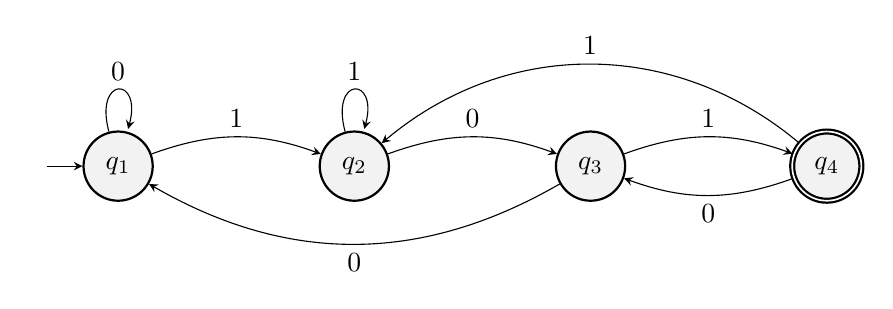
\begin{tikzpicture}
\node[state, initial] (q1) {$q_1$};
\node[state, right of=q1] (q2) {$q_2$};
\node[state, right of=q2] (q3) {$q_3$};
\node[state, accepting, right of=q3] (q4) {$q_4$};
\draw (q1) edge[loop above] node{0} (q1)
(q1) edge[bend left=20, above] node{1} (q2)
(q2) edge[loop above] node{1} (q2)
(q2) edge[bend left=20, above] node{0} (q3)
(q3) edge[bend left, below] node{0} (q1)
(q3) edge[bend left=20, above] node{1} (q4)
(q4) edge[bend right=40, above] node{1} (q2)
(q4) edge[bend left=20, below] node{0} (q3);
\end{tikzpicture}
\caption{Caption of the DFA $\mathcal{M}_1$}
\label{fig:my_label1}
\end{figure}

We can describe $\mathcal{M}_1$ formally by writing $\mathcal{M}_1 = (Q,\, \Sigma,\, \delta,\, q_1,\, F)$, where :
\begin{align*}
    &Q\,=\;\{q_1,\,q_2,\,q_3,\,q_4\},\;\text{the set of states}\\
    &\Sigma\,=\; \{ 0,\, 1 \}, \;\text{the binary alphabet}\\
    &F\,=\;\{q_4\},\; \text{the set of accepting states}\\
    &q_1\;\text{is the starting state}\\
    &\delta\,:\;Q\,\times\,\Sigma\,\to\,Q,\;\text{the transition function described as follows :}
\end{align*}

\begin{table}[H]
\renewcommand{\arraystretch}{1.25}
    \centering
    \begin{tabular}{|c||c|c|}
         \hline   
         &$0$&$1$  \\\hline\hline
         $q_1$&$q_1$&$q_2$  \\\hline
         $q_2$&$q_3$&$q_2$  \\\hline
         $q_3$&$q_1$&$q_4$  \\\hline
         $q_4$&$q_3$&$q_2$  \\\hline
    \end{tabular}
    \caption{$\mathcal{M}_1$\;Transition function}
    \label{tab:my_label1}
\end{table}

\noindent After a few trials, the language $\mathcal{L}(\mathcal{M}_1)$ recognized by the DFA seems to be :
\begin{align*}
    \mathcal{L}(\mathcal{M}_1)\,=\;\{w\in\Sigma^\star\,|\, \text{$w$ ends on "101"}\}.
\end{align*}
We denote an input string $x\in\Sigma^\star$, and $l$ its length. We prove by \textit{induction} on $l$ the following claim.
\paragraph{Claim} If the input string $x$ does not contain any “1” digits the $\mathcal{M}_1$ finishes in $q_1$, if $x$ ends on “00” and contains at least a “1” the $\mathcal{M}_1$ finishes in $q_1$, if $x$ ends on a “1” but does not contain “101” as a substring the $\mathcal{M}_1$ finishes in $q_2$, if $x$ ends on “10” the $\mathcal{M}_1$ finishes in $q_3$, if $x$ ends on a “1” after the last “101” substring the $\mathcal{M}_1$ finishes in $q_2$, and finally if $x$ ends on “101” the $\mathcal{M}_1$ finishes in $q_4$. Note that these 6 cases are mutually exclusive and every input falls into one of the cases.
\paragraph{Base case} If $l=0$ then $x$ is the empty string so it does not contain any “1” digits and indeed the $\mathcal{M}_1$ finishes in $q_1$ (the starting state) and the claim holds.
\paragraph{Induction hypothesis} Suppose that the claims is true for all $l<n$, where $n$ is an integer such that $n>0$.
\paragraph{Induction step} Let $l=n$ and let $x'$ be the first $n-1$ digits of $x$. Since the length of $x'$ is less than $n$, the induction hypothesis applies. We have 6 cases :
\begin{enumerate}
  \item Suppose $x'$ does not contain any “1” digits (by the induction hypothesis we are at $q_1$) and consider the last input digit $\sigma$. If $\sigma=$ “0”, $x$ does not contain any “1” digits either and indeed the $\mathcal{M}_1$ stays at $q_1$ and finishes. However if $\sigma=$ “1”, then $x$ ends on a “1” but does not contain “101” as a substring and indeed the $\mathcal{M}_1$ transitions to $q_2$ and finishes.
  \item Suppose $x'$ ends on “00” and contains at least a “1” (so by the induction hypothesis we are at $q_1$) and consider the last input digit $\sigma$. If $\sigma=$ “0”, $x$ still ends on “00” and contains at least a “1” and indeed the $\mathcal{M}_1$ stays at $q_1$ and finishes. However if $\sigma=$ “1”, then $x$ ends on a “1” and $x$ can either contain or not “101” as a substring, in both cases the $\mathcal{M}_1$ indeed transitions to $q_2$ and finishes.
  \item Suppose $x'$ ends on a “1” but does not contain “101” as a substring (so by the induction hypothesis we are at $q_2$) and consider the last input digit $\sigma$. If $\sigma=$ “0”, $x$ ends on “10” and indeed the $\mathcal{M}_1$ transitions to $q_3$ and finishes. However if $\sigma=$ “1”, then $x$ still ends on a “1” and does not contain “101” as a substring and indeed the $\mathcal{M}_1$ stays at $q_2$ and finishes.
  \item Suppose $x'$ ends on  “10” (so by the induction hypothesis we are at $q_3$) and consider the last input digit $\sigma$. If $\sigma=$ “0”, $x$ ends on “00” and contains at least a “1” and indeed the $\mathcal{M}_1$ transitions to $q_1$ and finishes. However if $\sigma=$ “1”, then $x$ ends on “101” and indeed the $\mathcal{M}_1$ transitions to $q_4$ and finishes.
  \item Suppose $x'$ ends on a “1” after the last “101” substring (so by the induction hypothesis we are at $q_2$) and consider the last input digit $\sigma$. If $\sigma=$ “0”, $x$ ends on “10” and indeed the $\mathcal{M}_1$ transitions to $q_3$ and finishes. However if $\sigma=$ “1”, then $x$ still ends on a “1” after the last “101” substring and indeed the $\mathcal{M}_1$ stays at $q_2$ and finishes.
  \item Suppose $x'$ ends on  “101” (so by the induction hypothesis we are at $q_4$) and consider the last input digit $\sigma$. If $\sigma=$ “0”, $x$ ends on “10” and indeed the $\mathcal{M}_1$ transitions to $q_3$ and finishes. However if $\sigma=$ “1”, then $x$ ends on a “1” after the last “101” substring and indeed the $\mathcal{M}_1$ transitions to $q_2$ and finishes.
\end{enumerate}

The hypothesis holds for $l=n$ and this completes the proof.


\section{Exercice 2}
\subsection{Probleme 2a}
For a language $\mathcal{L}\;\subseteq\;\Sigma^\star$, we define its \textit{triple} by :
\begin{align*}
    \mathcal{L}^3\;\coloneqq\;\{www :\,w\,\in\mathcal{L}\}
\end{align*}
Let us show that regular languages are \textit{not} closed under tripling. For that matter, we consider the following DFA, denoted $\mathcal{M}_2$ :

\begin{figure}[ht] % ’ht’ tells LaTeX to place the figure ’here’ or at the top of the page
\centering % centers the figure
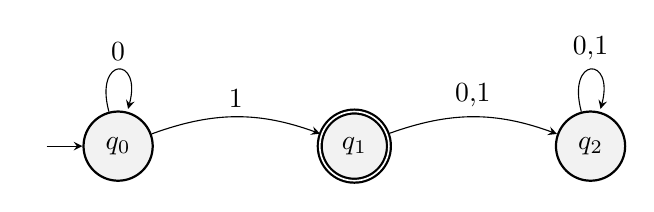
\begin{tikzpicture}
\node[state, initial] (q0) {$q_0$};
\node[state, accepting, right of=q0] (q1) {$q_1$};
\node[state, right of=q1] (q2) {$q_2$};
\draw (q0) edge[loop above] node{0} (q0)
(q0) edge[bend left=20, above] node{1} (q1)
(q1) edge[bend left=20, above] node{0,1} (q2)
(q2) edge[loop above] node{0,1} (q2);
\end{tikzpicture}
\caption{Caption of the DFA $\mathcal{M}_2$}
\label{fig:my_label2}
\end{figure}

We can describe this automaton formally by writing $\mathcal{M}_2 = (Q,\, \Sigma,\, \delta,\, q_0,\, F)$, where :
\begin{align*}
    &Q\,=\;\{q_0,\,q_1,\,q_2\},\;\text{the set of states}\\
    &\Sigma\,=\; \{ 0,\, 1 \}, \;\text{the alphabet}\\
    &F\,=\;\{q_1\},\; \text{the set of accepting states}\\
    &q_0\;\text{is the starting state}\\
    &\delta\,:\;Q\,\times\,\Sigma\,\to\,Q,\;\text{the transition function described as follows :}
\end{align*}

\begin{table}[H]
\renewcommand{\arraystretch}{1.25}
    \centering
    \begin{tabular}{|c||c|c|}
         \hline   
         &$0$&$1$  \\\hline\hline
         $q_0$&$q_0$&$q_1$  \\\hline
         $q_1$&$q_2$&$q_2$  \\\hline
         $q_2$&$q_2$&$q_2$  \\\hline
    \end{tabular}
    \caption{$\mathcal{M}_2$\;Transition function}
    \label{tab:my_label2}
\end{table}



Clearly, $\mathcal{M}_2$ recognizes the language :
\begin{align*}
    \mathcal{L}(\mathcal{M}_2)\,=\; \{0^n1\,|\, n\,\geq\, 0\},
\end{align*}
and $\mathcal{L}(\mathcal{M}_2)$ is regular.

Next we define the \textit{triple} $\mathcal{L}^3$ :
\begin{align*}
    \mathcal{L}^3\,=\;\{www :\,w\,\in\mathcal{L}(\mathcal{M}_2)\}\,=\,\{0^n10^n10^n1\,|\, n\,\geq\, 0\}.
\end{align*}

Suppose, for the sake of contradiction, that $\mathcal{L}^3$ is regular. Then we know that there must exist a positive integer $p$ satisfying the premises of the pumping lemma.

We pick $s$ $\coloneqq 0^p10^p10^p1\,\in\, \mathcal{L}^3$. According to the pumping lemma, there exists a split $s=xyz,\; \lvert xy\rvert\leq p,\, \lvert y\rvert\geq1$, such that for all $i\geq0,\; xy^iz\in\mathcal{L}^3$. Hence, we define $y\coloneqq0^k$, $1\leq k\leq p$. From the standpoint of the lemma, $\Tilde{s}\coloneqq xy^2z\in\mathcal{L}^3$, for $i=2$. However, the string $\Tilde{s}=0^{p+k}10^p10^p1$ and for any $k\in\Iintv{1,p}$, $\Tilde{s}$ is not the 3-time concatenation of the same string anymore.

Thus a contradiction is unavoidable if we make the assumption that $\mathcal{L}^3$ is regular, so $\mathcal{L}^3$ is \textit{not} regular. Quod Erat Demonstrandum.

\subsection{Probleme 2b}
Our purpose is to show that for a regular language $\mathcal{L}\subseteq\Sigma^\star$ over a \textit{unary alphabet}, $i.e.$ $\lvert\Sigma\rvert=1$, the \textit{triple} $\mathcal{L}^3$ as previously defined is regular.

Let $\mathcal{D}_1$ be a DFA such that :
\begin{align*}
    \mathcal{D}_1=(Q_1,\, \Sigma,\, \delta_1,\, q_1,\, F_1)
\end{align*} 
accepting the language $\mathcal{L}$ with $\lvert\Sigma\rvert=1$. In particular, we have : $F_1=\cup_{i=1}^{\lvert F_1\rvert}F_{1,i} $

Let $\mathcal{D}_{2,i}$ and $\mathcal{D}_{3,i}$ be copies of the DFA $\mathcal{D}_1$ such that :
\begin{align*}
    \mathcal{D}_{2,i}&=(Q_{2,i},\, \Sigma,\, \delta_{2,i},\, q_{2,i},\, F_{2,i})\quad\text{and}\\
    \mathcal{D}_{3,i}&=(Q_{3,i},\, \Sigma,\, \delta_{3,i},\, q_{3,i},\, F_{3,i})\quad\text{with}\quad i\in\Iintv{1,\lvert F_1\rvert}
\end{align*}

We modify every $\mathcal{D}_{2,i}$ and $\mathcal{D}_{3,i}$ such that the sets of accepting sets $F_{2,i}$ and $F_{3,i}$ contain only one accepting state $f_{2,i}$ and $f_{3,i}$ respectively, which corresponds to the $i$th final state.

Using the DFAs previously established, we create an NFA, denoted $\mathcal{N}$, such that :
\begin{align*}
    \mathcal{N}=(Q',\, \Sigma',\, \delta',\, q',\, F').
\end{align*}
We describe each of its components :
\begin{align*}
    Q'&=Q_1\cup \{\cup_{i=1}^{\lvert F_1\rvert}Q_{2,i}\}\cup \{\cup_{i=1}^{\lvert F_1\rvert}Q_{3,i}\}\quad\text{the states}\\
    \Sigma'&=\Sigma\quad\text{the}\;\textit{unary alphabet}\\
    q'&=q_1\quad\text{the starting state}\\
    F'&=\bigcup_{i=1}^{\lvert F_1\rvert}F_{3,i}\quad\text{the set of accepting sets}
\end{align*}
\begin{equation*}
    \delta'(q, a)=
    \begin{cases}
      \delta_1(q, a), & \text{if}\ q\in Q_1\;\text{and}\;q\notin F_1\\
      \delta_1(q, a), & \text{if}\ q\in F_1\;\text{and}\;a\neq\epsilon\\
      \delta_1(q, a)\cup\{q_{2,i}\}, & \text{if}\ q=f_{1,i}\;\text{and}\;a=\epsilon\\
      \delta_{2,i}(q, a), & \text{if}\ q\in Q_{2,i}\;\text{and}\;q\notin F_{2,i}\quad\quad\text{with}\quad i\in\Iintv{1,\lvert F_1\rvert}\\
      \delta_{2,i}(q, a), & \text{if}\ q\in F_{2,i}\;\text{and}\;a\neq\epsilon\\
      \delta_{2,i}(q, a)\cup\{q_{3,i}\}, & \text{if}\ q=f_{2,i}\;\text{and}\;a=\epsilon\\
      \delta_{3,i}(q, a), & \text{if}\ q\in Q_{3,i}\\
    \end{cases}
  \end{equation*}
  \\
  This completes our construction, and $\mathcal{L}^3$ is regular over a \textit{unary alphabet}. \\
  However, it is important to point out that all of this does not hold for any alphabet $\Sigma$, \textit{cf.} probleme 2a.
  \\\\
  %For instance, consider the following DFA with \textit{unary alphabet} ...
  %\textit{Caption of the DFA to be inserted.}\\\\which accepts $\mathcal{L}=...$ . The corresponding NFA for $\mathcal{L}^3$ is ... 
  %\textit{Caption of the NFA to be inserted.}
\end{document}
